% Options for packages loaded elsewhere
\PassOptionsToPackage{unicode}{hyperref}
\PassOptionsToPackage{hyphens}{url}
\PassOptionsToPackage{dvipsnames,svgnames,x11names}{xcolor}
%
\documentclass[
  letterpaper,
  DIV=11]{scrartcl}

\usepackage{amsmath,amssymb}
\usepackage{iftex}
\ifPDFTeX
  \usepackage[T1]{fontenc}
  \usepackage[utf8]{inputenc}
  \usepackage{textcomp} % provide euro and other symbols
\else % if luatex or xetex
  \usepackage{unicode-math}
  \defaultfontfeatures{Scale=MatchLowercase}
  \defaultfontfeatures[\rmfamily]{Ligatures=TeX,Scale=1}
\fi
\usepackage{lmodern}
\ifPDFTeX\else  
    % xetex/luatex font selection
\fi
% Use upquote if available, for straight quotes in verbatim environments
\IfFileExists{upquote.sty}{\usepackage{upquote}}{}
\IfFileExists{microtype.sty}{% use microtype if available
  \usepackage[]{microtype}
  \UseMicrotypeSet[protrusion]{basicmath} % disable protrusion for tt fonts
}{}
\makeatletter
\@ifundefined{KOMAClassName}{% if non-KOMA class
  \IfFileExists{parskip.sty}{%
    \usepackage{parskip}
  }{% else
    \setlength{\parindent}{0pt}
    \setlength{\parskip}{6pt plus 2pt minus 1pt}}
}{% if KOMA class
  \KOMAoptions{parskip=half}}
\makeatother
\usepackage{xcolor}
\setlength{\emergencystretch}{3em} % prevent overfull lines
\setcounter{secnumdepth}{-\maxdimen} % remove section numbering
% Make \paragraph and \subparagraph free-standing
\ifx\paragraph\undefined\else
  \let\oldparagraph\paragraph
  \renewcommand{\paragraph}[1]{\oldparagraph{#1}\mbox{}}
\fi
\ifx\subparagraph\undefined\else
  \let\oldsubparagraph\subparagraph
  \renewcommand{\subparagraph}[1]{\oldsubparagraph{#1}\mbox{}}
\fi


\providecommand{\tightlist}{%
  \setlength{\itemsep}{0pt}\setlength{\parskip}{0pt}}\usepackage{longtable,booktabs,array}
\usepackage{calc} % for calculating minipage widths
% Correct order of tables after \paragraph or \subparagraph
\usepackage{etoolbox}
\makeatletter
\patchcmd\longtable{\par}{\if@noskipsec\mbox{}\fi\par}{}{}
\makeatother
% Allow footnotes in longtable head/foot
\IfFileExists{footnotehyper.sty}{\usepackage{footnotehyper}}{\usepackage{footnote}}
\makesavenoteenv{longtable}
\usepackage{graphicx}
\makeatletter
\def\maxwidth{\ifdim\Gin@nat@width>\linewidth\linewidth\else\Gin@nat@width\fi}
\def\maxheight{\ifdim\Gin@nat@height>\textheight\textheight\else\Gin@nat@height\fi}
\makeatother
% Scale images if necessary, so that they will not overflow the page
% margins by default, and it is still possible to overwrite the defaults
% using explicit options in \includegraphics[width, height, ...]{}
\setkeys{Gin}{width=\maxwidth,height=\maxheight,keepaspectratio}
% Set default figure placement to htbp
\makeatletter
\def\fps@figure{htbp}
\makeatother

\KOMAoption{captions}{tableheading}
\makeatletter
\@ifpackageloaded{caption}{}{\usepackage{caption}}
\AtBeginDocument{%
\ifdefined\contentsname
  \renewcommand*\contentsname{Inhaltsverzeichnis}
\else
  \newcommand\contentsname{Inhaltsverzeichnis}
\fi
\ifdefined\listfigurename
  \renewcommand*\listfigurename{Abbildungsverzeichnis}
\else
  \newcommand\listfigurename{Abbildungsverzeichnis}
\fi
\ifdefined\listtablename
  \renewcommand*\listtablename{Tabellenverzeichnis}
\else
  \newcommand\listtablename{Tabellenverzeichnis}
\fi
\ifdefined\figurename
  \renewcommand*\figurename{Abbildung}
\else
  \newcommand\figurename{Abbildung}
\fi
\ifdefined\tablename
  \renewcommand*\tablename{Tabelle}
\else
  \newcommand\tablename{Tabelle}
\fi
}
\@ifpackageloaded{float}{}{\usepackage{float}}
\floatstyle{ruled}
\@ifundefined{c@chapter}{\newfloat{codelisting}{h}{lop}}{\newfloat{codelisting}{h}{lop}[chapter]}
\floatname{codelisting}{Listing}
\newcommand*\listoflistings{\listof{codelisting}{Listingverzeichnis}}
\makeatother
\makeatletter
\makeatother
\makeatletter
\@ifpackageloaded{caption}{}{\usepackage{caption}}
\@ifpackageloaded{subcaption}{}{\usepackage{subcaption}}
\makeatother
\ifLuaTeX
\usepackage[bidi=basic]{babel}
\else
\usepackage[bidi=default]{babel}
\fi
\babelprovide[main,import]{ngerman}
% get rid of language-specific shorthands (see #6817):
\let\LanguageShortHands\languageshorthands
\def\languageshorthands#1{}
\ifLuaTeX
  \usepackage{selnolig}  % disable illegal ligatures
\fi
\usepackage{bookmark}

\IfFileExists{xurl.sty}{\usepackage{xurl}}{} % add URL line breaks if available
\urlstyle{same} % disable monospaced font for URLs
\hypersetup{
  pdftitle={Mathematikprüfung},
  pdfauthor={Jonas Eggimann; Jonas Hunkeler},
  pdflang={de},
  colorlinks=true,
  linkcolor={blue},
  filecolor={Maroon},
  citecolor={Blue},
  urlcolor={Blue},
  pdfcreator={LaTeX via pandoc}}

\title{Mathematikprüfung}
\author{Jonas Eggimann \and Jonas Hunkeler}
\date{}

\begin{document}
\maketitle

\subsubsection{Angaben}\label{angaben}

Name, Niveau, Datum:

\begin{center}\rule{0.5\linewidth}{0.5pt}\end{center}

\subsubsection{Lernziele:}\label{lernziele}

Wir können:

\begin{itemize}
\tightlist
\item
  Längen mit Hilfe des Satzes von Pythagoras berechnen.
\item
  Objekte mit Zirkel und Lineal konstruieren.
\item
  mit Längen, Flächen und Volumen in Pyramiden rechnen.
\item
  mit Längen, Flächen und Volumen in geraden Prismen rechnen.
\end{itemize}

\begin{center}\rule{0.5\linewidth}{0.5pt}\end{center}

\subsubsection{Punkte}\label{punkte}

\begin{longtable}[]{@{}llllllll@{}}
\toprule\noalign{}
Aufgabe & 1 & 2 & 3 & 4 & 5 & 6 & \(\Sigma\) \\
\midrule\noalign{}
\endhead
\bottomrule\noalign{}
\endlastfoot
Punkte & 1 & 4 & 3 & 4 & 4 & 4 & 20 \\
\end{longtable}

Benötigte Anzahl Punkte für eine 6:

\begin{itemize}
\tightlist
\item
  16 (Real)
\item
  18 (Sek)
\item
  20 (Spez. Sek.)
\end{itemize}

\begin{center}\rule{0.5\linewidth}{0.5pt}\end{center}

\subsubsection{Hilfsmittel}\label{hilfsmittel}

Schreibzeug, Geodreieck, Lineal, Zirkel, Taschenrechner

\subsubsection{Allgemeine Hinweise}\label{allgemeine-hinweise}

Runde alle Zahlen auf zwei Nachkommastellen und notiere alle Resultate
mit einem Kugelschreiber. Alle Zahlenangaben geben wir als Längeneinheit
(LE) an. Sprich du musst keine Längeneinheit angeben.

\subsubsection{Zeit}\label{zeit}

45min

\subsubsection{Binnendifferenzierung}\label{binnendifferenzierung}

\begin{itemize}
\tightlist
\item
  Real-Niveau: Bei den Aufgaben mit einem (*) oder zwei Sternen (**)
  kannst du Bonuspunkte verdienen.
\item
  Sek-Niveau: Bei der Aufgabe mit zwei Sternen (**) kannst du
  Bonuspunkte verdienen.
\end{itemize}

Viel Glück

\begin{center}\rule{0.5\linewidth}{0.5pt}\end{center}

\subsection{Aufgabe 1}\label{aufgabe-1}

\href{https://be.lehrplan.ch/101PkqMkqzxUs36hHHkYEzbSuMg99acT6}{MA.2.A.3.h}

Kreuze die wahre Aussage an:

\begin{itemize}
\tightlist
\item
  Die Formel, um mit dem Satz des Pythagoras zu rechnen, lautet:
  \(a^2 + b^2 = c\)
\item
  DieFormel, um mit dem Satz des Pythagoras zu rechnen, lautet:
  \(a^2 + b^2 = c^2\)
\item
  Die Formel, um mit dem Satz des Pythagoras zu rechnen, lautet:
  \(1a^2 +1b^2 = 2c^2\)
\end{itemize}

\begin{center}\rule{0.5\linewidth}{0.5pt}\end{center}

\subsection{Aufgabe 2}\label{aufgabe-2}

\href{https://be.lehrplan.ch/101PkqMkqzxUs36hHHkYEzbSuMg99acT6}{MA.2.A.3.h}

Bestimme die fehlende Grösse der folgenden Dreiecke. Dein Rechnungsweg
muss ersichtlich sein.

\begin{figure}

\centering{

\captionsetup{labelsep=none}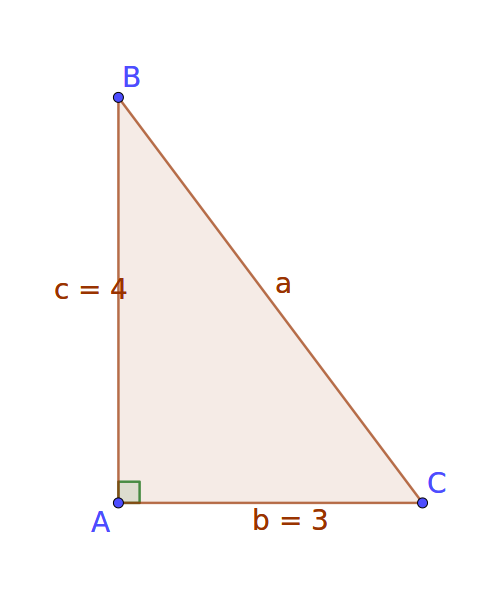
\includegraphics{math_07_geometrie_01_files/mediabag/images/geogebra-export.pdf}

}

\caption{\label{fig-aufgabe}}

\end{figure}%

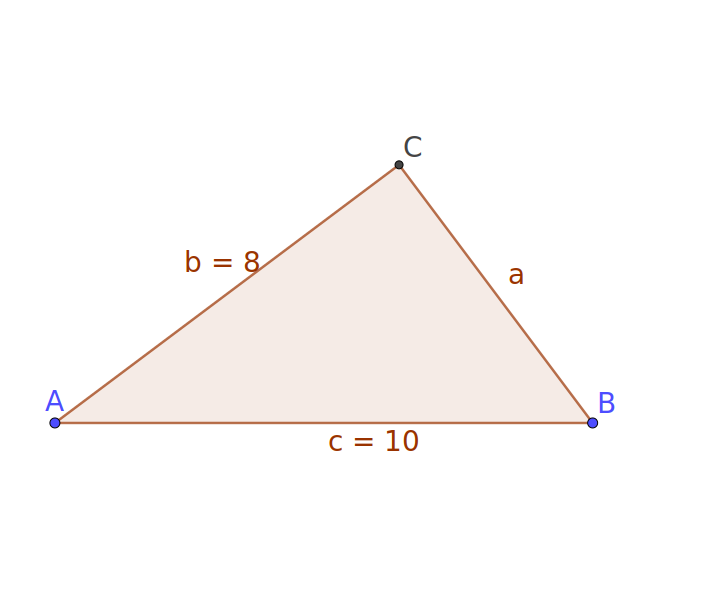
\includegraphics{math_07_geometrie_01_files/mediabag/images/geogebra-export_2.pdf}

\begin{center}\rule{0.5\linewidth}{0.5pt}\end{center}

\subsection{Aufgabe 3}\label{aufgabe-3}

\href{https://be.lehrplan.ch/101PkqMkqzxUs36hHHkYEzbSuMg99acT6}{MA.2.A.3.h}
\href{https://be.lehrplan.ch/101ynfPky7BFpr8TcpDdhJGF7bGBXERpT}{MA.2.A.1.i}

Bestimme vom gleichschenkligen Dreieck die Grundlinie \(g\).

Hinweis: Höhe des Dreiecks = 15

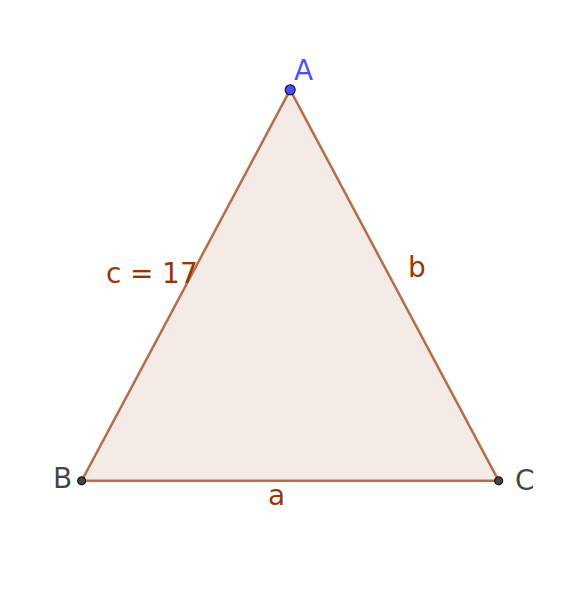
\includegraphics{math_07_geometrie_01_files/mediabag/images/geogebra-export_3.pdf}

\begin{center}\rule{0.5\linewidth}{0.5pt}\end{center}

\subsection{Aufgabe 4}\label{aufgabe-4}

\href{https://be.lehrplan.ch/101AWXeZS2HpzutW5DCGbwzdV7LxLJZWz}{MA.2.C.2.i}

Auftrag a*: Konstruiere die Mittelsenkrechte der Linie a.

Auftrag b**: Konstruiere mithilfe des Satzes von Thales ein
rechtwinkliges Dreieck. Hypotenuse = a

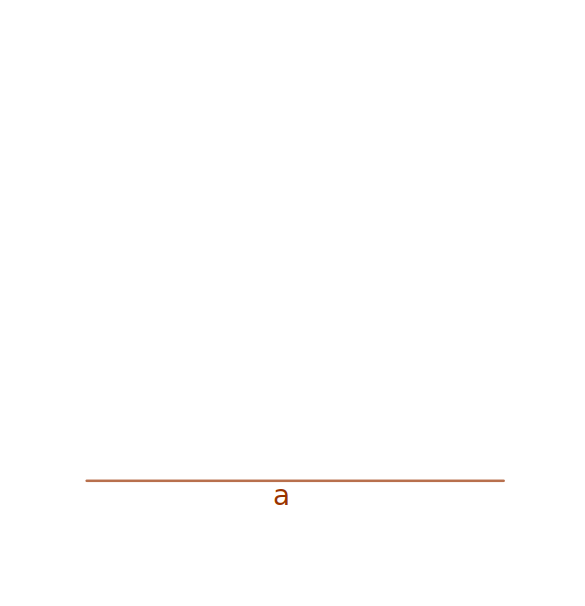
\includegraphics{math_07_geometrie_01_files/mediabag/images/geogebra-export_4.pdf}

\begin{center}\rule{0.5\linewidth}{0.5pt}\end{center}

\subsection{Aufgabe 5}\label{aufgabe-5}

\href{https://be.lehrplan.ch/101WHZAFydPBVsWSKRxVbDDTJ9S2qrXGZ}{MA.2.A.3.j}

Bestimme das Volumen und die Oberfläche der Pyramide. Hinweis:
gestrichelte Linie ist die Hälfte von a.

\(h = 6\) \(a = 4\)

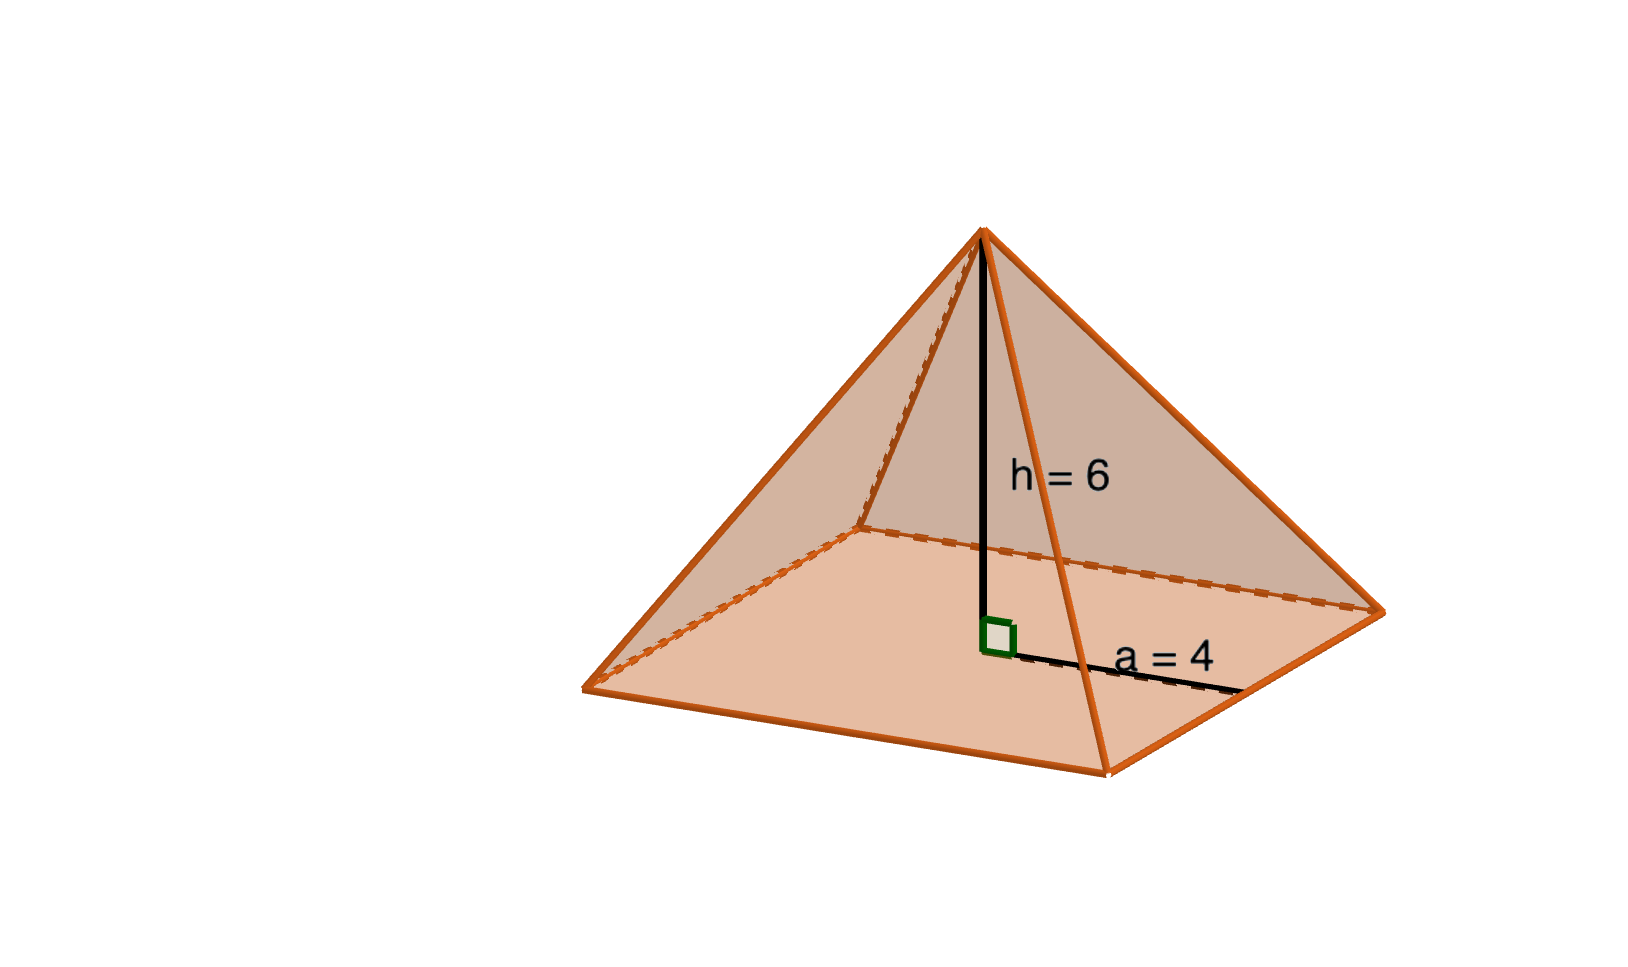
\includegraphics{images/geogebra-export_5.png}

\(V =\)

\(O =\)

\begin{center}\rule{0.5\linewidth}{0.5pt}\end{center}

\subsection{Aufgabe 6:}\label{aufgabe-6}

\href{https://be.lehrplan.ch/101bVuh6VdBgHN5Cz8e8GNuD4cNJh6x2p}{MA.2.A.1.k}
\href{https://be.lehrplan.ch/101hY2pesFLB3JJ6vSRYcnGYRen9Wuyfy}{MA.2.A.3.i}

\subsubsection{Auftrag (Real):}\label{auftrag-real}

Bestimme das Volumen und die

Oberfläche des Prismas. Gegeben: \(c = 10\) \(h_c = 4\) \(h_P = 12\)

\subsubsection{Auftrag (Sek):}\label{auftrag-sek}

Bestimme das Volumen und die Oberfläche des Prismas.

Gegeben: \(a = 12\) \(b = 8\) \(h_P = 22\)

\subsubsection{Auftrag (Spez-Sek):}\label{auftrag-spez-sek}

Bestimme das Volumen und die Oberfläche des Prismas.

Gegeben: \(a = 25\) \(c= 60\) \(h_P = 34\)

Volumen:

Oberfläche:

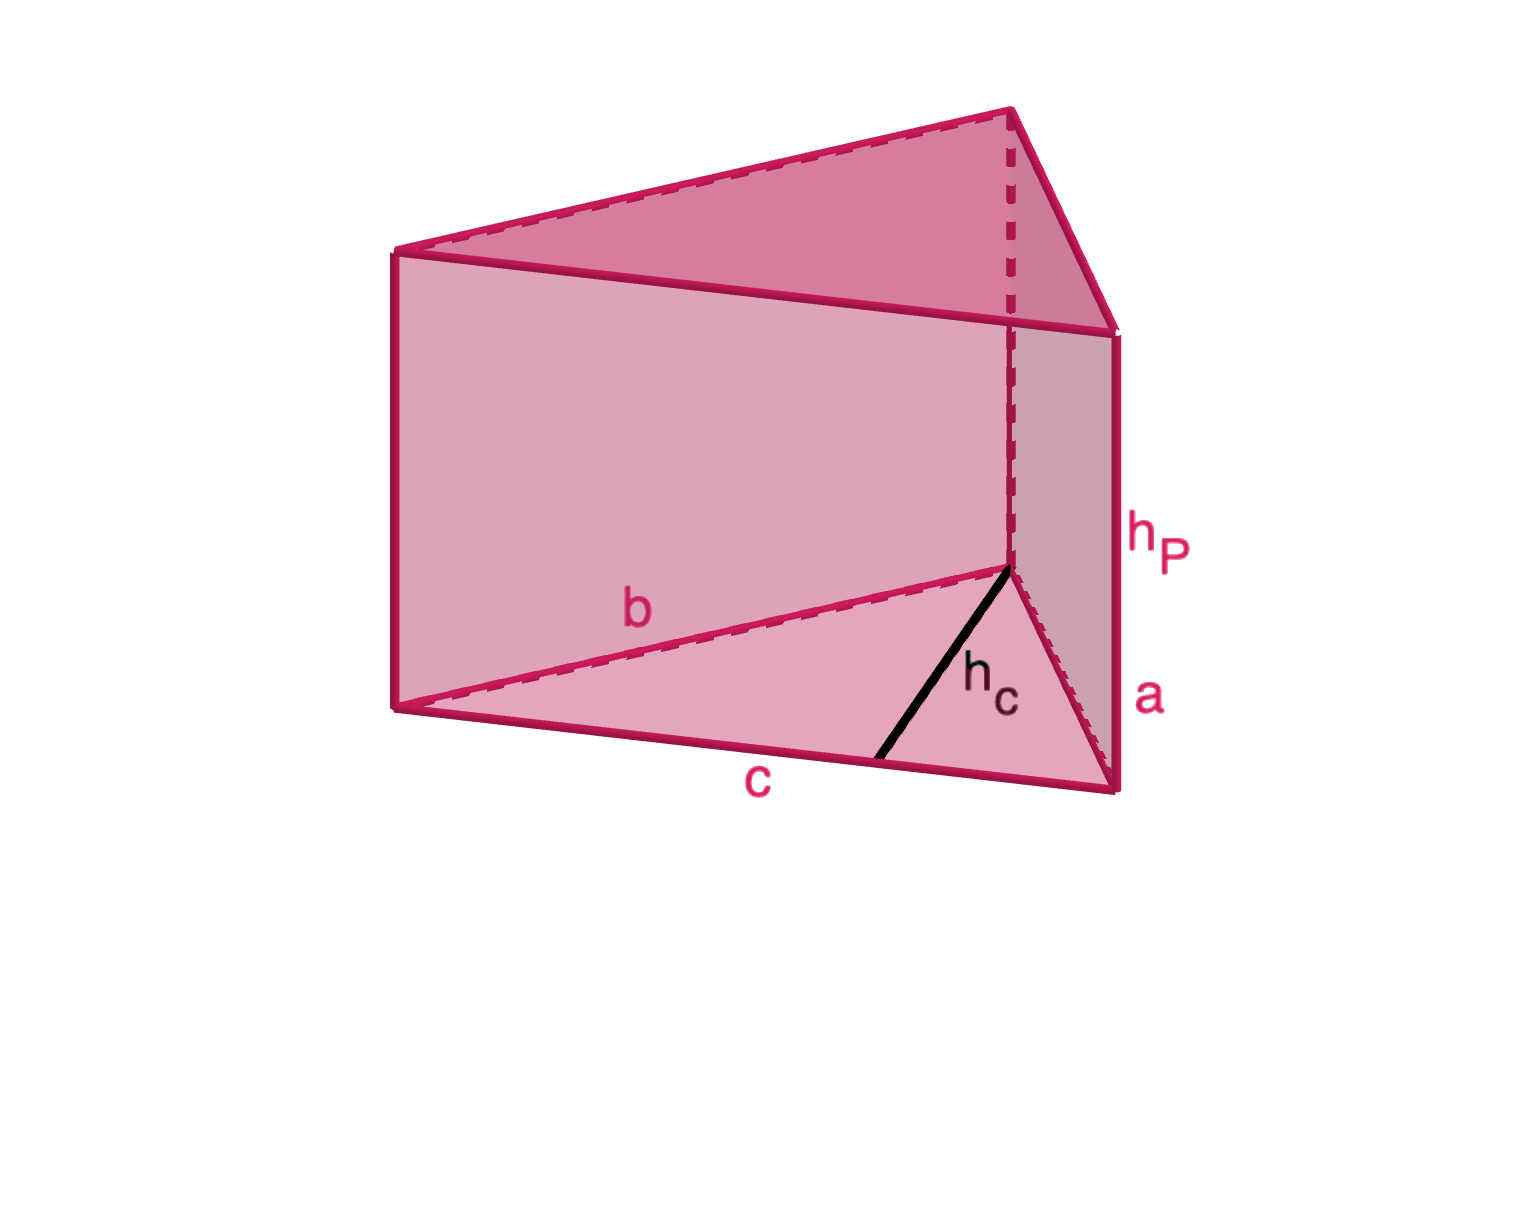
\includegraphics{images/geogebra-export_6.png}



\end{document}
